\documentclass[12pt]{ClasseMatematicamente}

\usepackage{graphicx}
\usepackage{amsmath}
\usepackage{amssymb}
\usepackage{verbatim} 
\usepackage{subfigure}
\usepackage{amsfonts}
%\usepackage{tikz}



\begin{document}

\pagestyle{fancy} \pagenumbering{arabic}


% --------------------------------------------------------------------

%---------  input heading  ------------
 \HeadingNumero{Numero 23}
 \HeadingData{Settembre 2014 - update \today ~- v0.0.1}
% %--------- input titolo -----------
 \NumeroArticolo{112}
 \Titolo{Hungarian algorithm: \\ a Short Presentation using Sage}
 
 \AutoreA{Sebastiano Ferraris}
 \EmailA{sebastiano.ferraris@gmail.com}

%%% ---  decommentare qui e nel .class le righe opportune per aggiungere altri autori (versione beta)

% \AutoreB{altroautore}
% \EmailB{altroautore@gmail.com}
 
% \AutoreC{altroautore}
% \EmailC{altroautore@gmail.com}
 
% \AutoreD{altroautore}
% \EmailD{altroautore@gmail.com}
 
% \AutoreE{altroautore}
% \EmailE{altroautore@gmail.com}

\Dedica{Dedicated to Federica Narciso, \\ to her courageous sweetness in life \\
and her tenacious talent in Mathematics.}
% %--------- input footing: numero di pagina di partenza ------------
\setcounter{page}{5}
% %----------------------------------------

\Issue

%\section*{Sommario}
%Qui mettere eventuale sommario ed introduzione

%------------ indice eventuale:
 %\tableofcontents
%____________________________


\noindent
The following pages are the result of sincere but disconcerted passion, some hours of spare time and the help of Luca Lussardi, Nicola De Nitti and Giuliano \lq\lq Nuanda\rq\rq \phantom{x}De Rossi. \\
This is to be intended as an introduction to the Hungarian Algorithm as well as a set of examples of recursive algorithms in Python. Any contribution, as suggestion, correction or improvement is welcome, so please do not hesitate to leave a comment or send me an email!

%%%%%%%%%%%%%%%%%%%%%%%%%%%%%%%%%%%%%%%%%%%%%%%%%%%%%%%%%%%%%%%%%%%%%%%%%%%%%%%
%%%%%%%
%%%%%%%%%%%%%%%%%%%%%%%%%%%%%%%%%%%%%%%%%%%%%%%%%%%%%%%%%%%%%%%%%%%%%%%%%%%%%%%
\section*{Introduction}\label{se:introduction}

Almost every article about Hungarian starts talking about associating worker and tasks. According to the tradition, imagine to be the manager of a manufacturing company and to have to decide the allocation of $4$ workers in $4$ different workstations. 
Every worker has different experiences and expresses a preference on the station in which he would like to work. The preference is expressed by giving a score from 1 to 20 (where 1 is the job that they prefer and 20 is the job they would like to avoid) \\
Your scope is to assign workers to workstations/tasks by making sure that everyone has a job close to its preference.\\
A way to find a solution to this problem, without comparing manually all the possibilities, is called \emph{Hungarian algorithm}. It was published by Harold Kuhn in $1955$, grounded on previous works made by two Hungarian mathematicians, Denes Konig and Jeno Egervary \cite{wiki}. In a more sophisticated perspective, not presented here, this problem can be seen as a particular application of the Hitchcock algorithm \cite{papadmitriou}.   

%%%%%%%%%%%%%%%%%%%%%%%%%%%%%%%%%%%%%%%%%%%%%%%%%%%%%%%%%%%%%%%%%%%%%%%%%%%%%%%%
\subsection*{Bipartite Matching}

A way to represent input data is using dots and connectors. Dots are used to represent both workers (Abigail, Baldwin, Cade, Diane) and tasks ($t1$, $t2$, $t3$, $t4$). Connectors to represent possible decisions between workers and tasks. 
\begin{figure}[!ht]
  \centering
  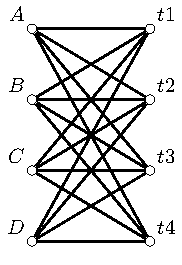
\includegraphics[height=7cm, width=4cm, angle=0,
   keepaspectratio]{figures/bipartite_graph_1.pdf}
  %\caption{Newspaper page with nodes and links}
  \label{fig:bipartite_graph}
\end{figure}
\noindent
We assign to each connector a value corresponding to the score given by each worker to the connected task: if Abigail gives a score to the task $t1$ equals to $15$, then the value of the connector from $A$ to $t1$ will be $15$. \\ 
Models made by dots and connectors are in general called \emph{graphs}, dots are called \emph{nodes} and connectors are called \emph{edges}. Graph used in this situation are called \emph{bipartite complete graph}. In the first partition we have workers and in the second partition we have tasks \cite{grafi}.
The number associated to each edge is called \emph{weight of the edge}. \\
In general, given two sets $A$ and $B$ with the same number of elements $n = \vert A \vert = \vert B \vert$, for which is defined a \emph{weight function} $w$,

\begin{align*}
  w : A \times B  &\longrightarrow  \mathbb{R}_{+} \\
   (a,b) &\longmapsto w(a,b) 
\end{align*}
such that for every couple $(a,b)$ it associates a positive value,
it is always possible to draw a corresponding bipartite complete graph
\footnote{You may have to take your time to unpack this sentence. If $X$ is a set, the number of its elements is written as $\vert X \vert$ and it is called cardinality of $X$. $A \times B$ is the cartesian product of the set $A$ times the set $B$ and it is the domain of the function $w$. The range of the function is the set of positive real numbers $ \mathbb{R}_{+}$, the arrow $\mapsto$ means that the element $(a,b)$ of the domain is mapped into $w(a,b)$.}. 
A subset of edges with no common nodes is called \emph{matching}. A matching in a bipartite complete graph with $n$ nodes in each partition is \emph{maximal} if you cannot add an edge to the matching while keeping the condition of not having common nodes for each edge. To each maximal matching corresponds a possible assignment workers-tasks. \\
In the figure below the maximal matching is highlighted in blue with the weight of the choose arch. 

\noindent
Abigail is assigned to the job $t2$ (score $16$), Baldwin to the $t3$ (score $2$), Cade to the $t1$ (score $17$) and Diane to $t4$ (score $14$).
The \emph{weight of the matching} is the sum of the weights of the edges involved (in this case it is 49).
Our aim is to find the maximal matching with minimal weight, i.e. to solve the so called \emph{matching problem}.

\begin{figure}[!ht]
	\centering
	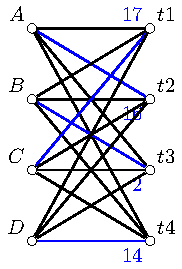
\includegraphics[height=7cm, width=4cm, angle=0,
	keepaspectratio]{figures/bipartite_graph_2.pdf}
	\label{fig:bipartite_graph_blue}
\end{figure}
\begin{figure}[!ht]
	\centering
	\includegraphics[height=10cm, width=10cm, angle=0,
	keepaspectratio]{figures/dia_main_1.png}
	\caption{Hungarian Algorithm Flowchart}
	\label{fig:main_flow}
\end{figure}


%%%%%%%%%%%%%%%%%%%%%%%%%%%%%%%%%%%%%%%%%%%%%%%%%%%%%%%%%%%%%%%%%%%%%%%%%%%%%%%%
\subsection*{Cost Matrix}
The representation of data with bipartite graph could be enough to reach the solution with a straight strategy, involving a device called \emph{augmenting path}\footnote{This way is well presented in \cite{mordecai}.}. In the solution to the matching problem that is presented here, the bipartite graph is not enough, and a second tool is necessary: the \emph{cost matrix}. \\
Consider the set of employees as a vector in alphabetical order $\mathbf{e} = (A,B,C,D)$ and the vector of tasks ordered as $\mathbf{t}=(t1,t2,t3,t4)$; the \emph{cost matrix} is defined as follows
\begin{align*}
  M[i,j] = w(\mathbf{e}[i],\mathbf{t}[j]) 
\end{align*}
Where $w(\mathbf{e}[i],\mathbf{t}[j])$ is the score that the worker $\mathbf{e}[i]$ gives to $\mathbf{t}[j]$.\\
In our leading example we will consider:
\begin{equation}\label{matrix_M}
M = 
\left(\begin{array}{rrrr}
15 & 16 & 19 & 4 \\
6 & 1 & 2 & 6 \\
17 & 3 & 5 & 12 \\
13 & 6 & 16 & 14
\end{array}\right)
\end{equation}
At the position $[1,0]$ of $M$ we find\footnote{According to Python language, indexes start from zero: $M[1,0]$ is the elment in the second row and in the firs column of $M$.} the score of Baldwin for the job $t1$, which is equal to $6$. 
A set of $n$ of elements of the cost matrix, such that none of them are on the same row or in the same vector corresponds to a matching. The association presented in the above figure can be represented in the cost matrix with bold numbers:
$$
M = 
\left(\begin{array}{rrrr}
15 & \mathbf{16} & 19 & 4 \\
6 & 1 & \mathbf{2} & 6 \\
\mathbf{17} & 3 & 5 & 12 \\
13 & 6 & 16 & \mathbf{14}
\end{array}\right)
$$
It is easy to see that the set of the feasible solutions, i.e. the possible associations, has $4!$ elements ($4$ possible on the first row, $3$ on the second, $2$ on the third). Each feasible solution can be represented in the most economical way with a vector $\mathbf{s}$ of dimension $4$, such that in the first position we find the index of the column of the choose element in the first row of $M$. In the second position, the index of the column of the element in the second row of $M$ and so on.
In the previous case the vector corresponding to the matching is:
\begin{align*}
 \mathbf{s} = (1,2,0,3)
\end{align*} 
The \emph{space of the feasible solution} $\mathcal{F}$ is the set of the vectors of dimension $4$ containing numbers in the set $\lbrace 0,1,2,3\rbrace $ with no repetitions.\\
The \emph{cost} of a vector $\mathbf{s}$ in $\mathcal{F}$ is defined as 
\begin{align*}
 w(\mathbf{s}) = \sum_{i=0}^{3} M[i,\mathbf{s}[i]]
\end{align*}
and it corresponds to the weight of the matching.\\
The solution we are searching for is a vector in the set $\mathcal{F}$ with minimal cost (it is called \emph{solution vector} and it may be not unique). Since $\mathcal{F}$ has $n!$ elements, it is inconvenient to employ a brute force algorithm to find it.


%%%%%%%%%%%%%%%%%%%%%%%%%%%%%%%%%%%%%%%%%%%%%%%%%%%%%%%%%%%%%%%%%%%%%%%%%%%%%%%%
%%%%%%%%%%%%%%%%%%%%%%%%%%%%%%%%%%%%%%%%%%%%%%%%%%%%%%%%%%%%%%%%%%%%%%%%%%%%%%%
\section*{Step by Step Algorithm}\label{se:stepbystep}
We propose a version of the algorithm which uses 4 main functions (\emph{row reduction}, \emph{column reduction}, \emph{percolation finder}, \emph{shaker}, \emph{resolvability test}), and 2 auxiliary function (\emph{covering segments searcher} and \emph{redundance filter}).
The \emph{input} of the algorithm is the cost matrix $M$ (it contains all information we need to solve the problem) and the \emph{output} is the solution vector.
In the following subsections each step is presented separately with Sage implementation and examples. 

%%%%%%%%%%%%%%%%%%%%%%%%%%%%%%%%%%%%%%%%%%%%%%%%%%%%%%%%%%%%%%%%%%%%%%%%%%%%%%%%
\subsection*{Step 1: Row Reduction}
The step 1 consists of the application of a function which finds the minimal element to each row and subtract it to all the elements of the row.

\begin{small}
\begin{lstlisting}
def row_reduction(m):
	"""
	step 1: row reduction
	:param m input matrix (type np.matrix)
	:return: m after row reduction: for each row the minimal element 
	         is subtracted to each element of the row
	"""
	assert isinstance(m, np.matrixlib.defmatrix.matrix)
	return m - np.min(m, axis=1)
\end{lstlisting}
\end{small}


%%%% Esempio step 1  
\noindent
The first line of the code asserts that m is an instance of the class np.matrix. If not the behaviour of np.min would change.
The matrix \ref{matrix_M} is provided to an ipython session as follows:
\begin{small}
\begin{lstlisting}
import numpy as np  # importing the library numpy 
M = np.matrix([[15,16,19,4],[6,1,2,6],[17,3,5,12],[13,6,16,14]]); M
\end{lstlisting}
\end{small}
$$
\left(\begin{array}{rrrr}
15 & 16 & 19 & 4 \\
6 & 1 & 2 & 6 \\
17 & 3 & 5 & 12 \\
13 & 6 & 16 & 14
\end{array}\right)
$$
\begin{small}
 \begin{verbatim}
M1 = row_reduction(M); M1
\end{verbatim}
\end{small}
$$
\left(\begin{array}{rrrr}
11 & 12 & 15 & 0 \\
5 & 0 & 1 & 5 \\
14 & 0 & 2 & 9 \\
7 & 0 & 10 & 8
\end{array}\right)
$$

%%%%%%%%%%%%%%%%%%%%%%%%%%%%%%%%%%%%%%%%%%%%%%%%%%%%%%%%%%%%%%%%%%%%%%%%%%%%%%%%
\subsection*{Step 2: Column Reduction}
Step 2 refers to the columns: for each column it finds the minimal element and subtract it to all of the elements of the column. 

\begin{small}
\begin{lstlisting}
def col_reduction(m):
	"""
	step 2: row reduction
	:param m input matrix (type np.matrix)
	:return: m after col reduction: for each column the minimal element 
	is subtracted to each element of the column
	"""
	assert isinstance(m, np.matrixlib.defmatrix.matrix)
	return m - np.min(m, axis=0)
\end{lstlisting}
\end{small}


%%%% Esempio step 1
\noindent
Applying this in our leading example we get:
\begin{small}
 \begin{verbatim}
M2 = col_reduction(M1); M2
\end{verbatim}
\end{small}
\begin{equation}\label{matrix_M2}
\left(\begin{array}{rrrr}
6 & 12 & 14 & 0 \\
0 & 0 & 0 & 5 \\
9 & 0 & 1 & 9 \\
2 & 0 & 9 & 8
\end{array}\right)
\end{equation}
The solution vector does not change if we consider $M$ or $M$ after having applied row or column reduction. 
\begin{lemma}
 Let $\mathbf{s}_1$ and $\mathbf{s}_2$ two vectors in the space of feasible solutions, $w$ the weight function defining $M$ and $\hat{w}$ the weight function defining $row\textunderscore reduction(M)$. If $w(\mathbf{s}_1) \leq w(\mathbf{s}_2)$ then $\hat{w}(\mathbf{s}_1) \leq \hat{w}(\mathbf{s}_2)$.
\end{lemma}
\begin{proof}
 Let $m_{i}$ the min in the $i$-th row. Subtract $m_{i}$ to the $i$-th row is the same as subtract it to each edge with a common node of the first partition in the related bipartite complete graph. If $w_{i}$ is the weight function defined by the matrix where we have subtracted the $m_{i}$ only in the $i$-th row we have $w_{i}(\mathbf{s}) = w(\mathbf{s}) - m_{i}$.\\
 It follows that $\hat{w}(\mathbf{s}) = w(\mathbf{s}) - \sum_{i=0}^{n-1} m_{i}$ for each $\mathbf{s}$ in the feasible space.
\end{proof}
It can be shown that the lemma is still valid if $\hat{w}$ is the weight function of $col\textunderscore reduction(M)$. It follows then:
\begin{theor}
 The solution vector for the matrix $M$ is the same as for the matrix \\
 $col\textunderscore reduction(row\textunderscore reduction(M))$ as well as for the matrix 
 $row\textunderscore reduction(col\textunderscore reduction(M))$.
\end{theor}
Note that in general $col\textunderscore reduction(row\textunderscore reduction(M)) \neq row\textunderscore reduction(col\textunderscore reduction(M))$. Which means that you may not get the same matrix if the order of application of step 1 and step 2 is inverted.

%%%%%%%%%%%%%%%%%%%%%%%%%%%%%%%%%%%%%%%%%%%%%%%%%%%%%%%%%%%%%%%%%%%%%%%%%%%%%%%%
\subsection*{Step 3: Percolation Finder}

After step 1 and 2 we have got a matrix with some zeros (at least one for each row and one for each column). If it is possible to \lq\lq walk\rq\rq\phantom{z}the matrix from the first row to the last just stepping on zeros and never passing twice on the same column, our walk will be the solution vector we are searching for, and we are done with the Hungarian Algorithm!\\

\noindent
For example in the following matrix 
$$
N = 
\left(\begin{array}{rrrr}
6 & 11 & 0 & \mathbf{0} \\
12 & \mathbf{0} & 0 & 4 \\
\mathbf{0} & 15 & 5 & 1 \\
8 & 14 & \mathbf{0} & 1
\end{array}\right)
$$
we can see such kind of walk and we can notice that the solution is $\mathbf{s} = (3,1,0,2)$. In the matrix (\ref{matrix_M2}) of the main example, a possible walk through zeros corresponds to the vector $(3,2,1,1)$ which is not a feasible solution. \\

\noindent
This rough idea of walk can be formalized under the name of percolation: 
\begin{definition}
Given a costs matrix $M$, a {\bf percolation} over $M$ is a subset of $n$ element of the matrix $M$, one and only one for each row. If all the elements of a percolation are zeros, it is called $0$-{\bf percolation}.
\end{definition}
As just seen, not all the matrices admits $0$-percolation, but it easy to prove that every output of step 1 and step 2 admits at least one. \\
As made in our example we can identify every $0$-percolation with a vector $\mathbf{v} = (j_1, j_2, \dots , j_n)$ of dimension $n$ made of integer in the set $\lbrace 0,1,2, \dots, n-1 \rbrace$. With this nomenclature if $\mathbf{v}[i] = j_i$ then the element $M[i,j_i]$ belongs to the percolation. 
For example in the matrix $N$, $4$ $0$-percolations are possible:
$$
\left(\begin{array}{rrrr}
6 & 11 & \mathbf{0} & 0 \\
12 & \mathbf{0} & 0 & 4 \\
\mathbf{0} & 15 & 5 & 1 \\
8 & 14 & \mathbf{0} & 1
\end{array}\right)
\qquad
\left(\begin{array}{rrrr}
6 & 11 & 0 & \mathbf{0} \\
12 & \mathbf{0} & 0 & 4 \\
\mathbf{0} & 15 & 5 & 1 \\
8 & 14 & \mathbf{0} & 1
\end{array}\right)
\qquad
\left(\begin{array}{rrrr}
6 & 11 & \mathbf{0} & 0 \\
12 & 0 & \mathbf{0} & 4 \\
\mathbf{0} & 15 & 5 & 1 \\
8 & 14 & \mathbf{0} & 1
\end{array}\right)
\qquad
\left(\begin{array}{rrrr}
6 & 11 & 0 & \mathbf{0} \\
12 & 0 & \mathbf{0} & 4 \\
\mathbf{0} & 15 & 5 & 1 \\
8 & 14 & \mathbf{0} & 1
\end{array}\right)
$$
The first, third and fourth do not represent a feasible solution as two zeros involved in the 0-percolation are in the same column.
It is interesting to count how many zeros of the same $0$-percolation are in the same column, since the solution we are searching for will be the $0$-percolation having exactly $1$ zero in each column: the second 0-percolation emphasised in the previous example.

\noindent
The mathematical tool that states how far is our percolation from the one that we are searching lies in the following definition:
\begin{definition}
 Given a $0$-percolation $\mathbf{v}$ over $M$ of length $n$, the index of redundancy of $\mathbf{v}$ is a real number defined as the maximal number of zeros of the percolation in the same column minus 1, plus the number of columns with no elements in the 0-percolation divided by the length of the percolation.
\end{definition}
Sometimes a formula can make a definition easier to be understand. This is one of this cases:
\begin{align*}
 \text{index\textunderscore of\textunderscore redundancy}(\mathbf{v}) 
 =& 
 \text{~max (zeros of the percolation in the same column)} -1 +\\
 &+ |\{ \text{columns with no elements in the 0-percolation} \} | /n
\end{align*}
where max is the maximal number of zeros of the percolation in the same column.\\
In the previous example we have
$$
\begin{array}{l l l l }
 (2,1,0,2)~1.25\qquad\qquad & (3,1,0,2)~0 \qquad\qquad & (2,2,0,2)~2.5 \qquad\qquad & (3,2,0,2)~1.25 
\end{array}
$$
where each index of redundancy is shown on the right of its percolation. 
Given the percolation $V$ a function to calculate the redundancy index is:

\begin{small}
\begin{lstlisting}
def redundace_index(v):
	"""
	step 3: redundacy index
	"""
	n = v.size
	occurrence_vector = [v.count(i) for i in range(n)]
	return np.max(occurrence_vector) - 1 + occurrence_vector.count(0) / float(n)
\end{lstlisting}
\end{small}

\noindent
where \emph{occurrence vector} at the position $i$ gives the number of occurrence of the number $i$ in the vector $V$.
If $M$ admits at leas one $0$-percolation with redundancy index equals to $0$, a recursive\footnote{An introduction to recursive algorithm can be found in \cite{sedgewick}.} algorithm to find it, can be:
\begin{small}
\begin{lstlisting}
ans = []

def percolation_finder_0(M):
	"""
	percolation finder initial version
	:param M: cost matrix after col and row reduction.
	:return: True if the matrix admits a 0-percolation with redundancy 
	index equals to 0, False otherwise. 
	In the global variable ans is recorded the first 0-percolation found if it  exists. 
	"""
	def find_walk(M, row, sol):
		global ans
		print(row)
		for i in range(M.shape[1]):
			if M[row, i] == 0 and i not in sol:
				sol = sol + [i]
				ans = sol
				#print(ans)
				if row >= M.shape[1] - 1 or find_walk(M, row+1, sol):
					return True                    
				else:
				sol = sol[0:-1] 
		return False 
	return find_walk(M, 0, [])
\end{lstlisting}
\end{small}

\noindent
Uncommenting the line \emph{print ans} allows to see the recursive algorithm at work. Note that to use this algorithm twice in the same session, you must initialize the global variable to the empty list.
If the matrix has more than one solution, the previous algorithm provides us only the first that he finds, stored in the variable $ans$. In general the matrix could admit no solution at all. In this case all the $0$-percolation have redundancy index grater then $0$.\\ 
This means that we have identified the following two cases:
\begin{enumerate}
 \item $row\textunderscore reduction(col\textunderscore reduction(M))$ admits $0$-percolation with redundancy index equals to $0$.
 \item $row\textunderscore reduction(col\textunderscore reduction(M))$ does not admit any $0$-percolation with redundancy index equals to $0$.
\end{enumerate}
We need an algorithm that provides {\bf all} the $0$-percolation and tells if some of them has index of redundancy equals to zero or not, as this will be our solution. 
We use again recursion:


\begin{small}
\begin{lstlisting}
	def percolation_finder_1(m, max_num_percolation=6):
		"""
		percolation finder initial version 1
		:param m: cost matrix m.
		:param max_num_percolation: maximal number of 0-percolations returned.
		:return: list of all of the 0-percolation, up to max_num_percolation, followed by redundancy index.
		"""
		walks = { 'walk': [] }  # Name binding
		
		def scout(m, breadcrumbs):
			ncols = m.shape[1]
			crumbs_number = len(breadcrumbs)
			
			#print(breadcrumbs)
			if crumbs_number < ncols:
				for j in range(ncols):
					if m[crumbs_number,j] == 0:
						scout(m,breadcrumbs + [j])
			elif crumbs_number == ncols:
				walks['walk'] = walks['walk'] + [breadcrumbs]
		
		for j in range(m.shape[1]):
			if m[0,j] == 0:
				scout(m, [j])
		return walks['walk']
\end{lstlisting}
\end{small}


\noindent
As before, uncommenting the line \emph{print breadcrumbs}, we can see recursion at work. You may have noticed that a matrix with a lots of zeros makes the walks list too big to be manageable.
Since we are not interested in all the percolation but only in those with minimal redundancy, we add a strategy to decide if we may want to stop after having collected \lq\lq enough\rq\rq\phantom{z}percolations in the vector \emph{walks}:


\begin{small}
\begin{lstlisting}
def percolation_finder(m, max_num_percolation=6):
	"""
	Step 3 percolation finder
	:param m: cost matrix m.
	:param max_num_percolation: maximal number of 0-percolations returned.
	:return: list of all of the 0-percolation, up to max_num_percolation, 
	         followed by redundancy index.
	"""
	walks = { 'walk': [] }  # Name binding
	
	def redundancy_index(v):
		n = len(v)
		occurrence_vector = [v.count(i) for i in range(n)]
		return max(occurrence_vector) - 1 + occurrence_vector.count(0) * 1.0 / n
	
	def scout(m, breadcrumbs):
		n_cols = m.shape[0]
		crumbs_number = len(breadcrumbs)
		# print(breadcrumbs)
		if crumbs_number < n_cols:
			col_index_arranged = list(set(range(n_cols)) - set(breadcrumbs)) + \
			                     list(set(breadcrumbs))
			for j in col_index_arranged:
				if m[crumbs_number, j] == 0:
					# More scouts are launched only if some place in the walks' 
					# vector is available. Rearranging indexes may guarantee 
					# that a percolation with 0 redundancy index is stored in the
					# first explorations, when available.
					if len(walks['walk']) < 2 * max_num_percolation:
						scout(m, breadcrumbs + [j])
		elif crumbs_number == n_cols:
			walks_recorder(breadcrumbs)
	
	def walks_recorder(v):
		ri = redundancy_index(v)
		walks['walk'] = walks['walk'] + [v] + [ri]
		
	first_zero = True
	for j in range(m.shape[1]):
		if m[0, j] == 0:
			if first_zero:
				# reset to [] the list of walks
				walks['walk'] = []
				first_zero = False
			#print('A scout goes in mission')
			scout(m, [j])
	
	if len(walks['walk']) == 0:
		raise TypeError('Input matrix has no 0-percolations.')
	
	return [m, walks['walk']]
\end{lstlisting}
\end{small}


\noindent
The function \emph{walks\textunderscore recorder} adds to the global variable \emph{walks} each new $0$-percolation followed by its redundance index \emph{ri}.
If the variable \emph{find\textunderscore all}, in the input value, is set to \emph{False} then the vector walks will collect only a number of $0$-percolation equals to \emph{max\textunderscore percolation}.\footnote{Note that this just stop the recording, and do not stops the recursive steps. It is also possible to stop the recursion when the \emph{max \textunderscore percolation} is reached. This option is not proposed here for clarity.} It does make sense to stop the recursion before all $0$-percolation are collected, just because the indexes of the first cycle-for had been rearranged:
\begin{small}
\begin{lstlisting}
col_index_arranged = list(set(range(ncols))-set(breadcrumbs)) + list(set(breadcrumbs))
\end{lstlisting}
\end{small}
This means that when the algorithm is arrived at the row \emph{crumbs\textunderscore number} it searches for a new zero before in columns that have not been used already. For example, if the input matrix is like the following (the best case to find a solution as well as one of the worst case for a recursive algorithm) 
$$
N = 
\left(\begin{array}{rrrr}
0 & 0 & 0 & 0 \\
0 & 0 & 0 & 0 \\
0 & 0 & 0 & 0 \\
0 & 0 & 0 & 0
\end{array}\right)
$$
the first $0$-percolation that the algorithm finds is the solution $(0,1,2,3)$. So it makes sense to limit the solution, even thought if the number \emph{max\textunderscore percolation} is too little we may lose some multiple solution.\\
Applying this to our main example (matrix \ref{matrix_M2}) we get:
\begin{small}
\begin{lstlisting}
walks 
[[3, 0, 1, 1], 1.25, [3, 1, 1, 1], 2.5, [3, 2, 1, 1], 1.25]
\end{lstlisting}
\end{small}

%%%%%%%%%%%%%%%%%%%%%%%%%%%%%%%%%%%%%%%%%%%%%%%%%%%%%%%%%%%%%%%%%%%%%%%%%%%%%%%%
\subsection*{Step 4: Resolvability Query}
At this stage we have got the matrix reduced and the list of $0$-percolation (complete or not) with related redundancy indexes. 
After the step $4$ we will have the list of $0$-percolation with minimal redundancy index, and a flag which states if the $0$-percolation (or percolations) found is already our solution or not.

\begin{small}
\begin{lstlisting}
def resolvability_query(m, walks_):
	"""
	:param m: cost matrix
	:param walks_: list of 0-percolation followed by its index of redundancy
	as returned by percolation_finder
	:return: M again untouched, followed by the list of $0$-percolation with
	minimal index of redundancy, and with a flag, True if the minimal index
	is 0 and so we have already our solution, False otherwise.
	"""
	min_redundancy = np.min(walks_[1::2])
	filtered_walks = [walks_[i] for i in list(range(len(walks_)))[::2] \
			          if walks_[i + 1] == min_redundancy]
	if min_redundancy == 0:
		flag = True
	else:
		flag = False
	return [m, filtered_walks, flag]

\end{lstlisting}
\end{small}

The iterator (or list in python 2) $range(len(walks))[::2]$ is the list of the redundancy index in the vector walks (all the odd position in the vector).\\
Lets see it at work on our main example:
\begin{small}
 \begin{lstlisting}
A,B = percolation_finder(M2); A,B
resolvability_query(A,B)
\end{lstlisting}
\end{small}
\begin{equation}\label{matrix_M4}
\left[\left(\begin{array}{rrrr}
6 & 12 & 14 & 0 \\
0 & 0 & 0 & 5 \\
9 & 0 & 1 & 9 \\
2 & 0 & 9 & 8
\end{array}\right), \left[3, 0, 1, 1\right], \left[3, 2, 1, 1\right],
\mathrm{False}\right]
\end{equation}
When the flag is True the job is done. If it is False we must do some manipulation on the matrix in order to add some zeros without change the results. This tricky passage is here the step number $5$, called shaker.

%%%%%%%%%%%%%%%%%%%%%%%%%%%%%%%%%%%%%%%%%%%%%%%%%%%%%%%%%%%%%%%%%%%%%%%%%%%%%%%%
\subsection*{Step 5: Shaker}

To perform this passage, first of all we must find the \emph{covering segments} of the input matrix $M$. A covering of $M$ is the minimal set of horizontal or vertical segments that covers all the zeros in the matrix. In \cite{sito_1}, it is suggested to actually draw horizontal or vertical lines over the matrix, covering all the zeros such that the number of lines is minimal.
Here, instead of using covering segments, we use a couple of vectors called \emph{covered\textunderscore col} and \emph{covered\textunderscore row}:
\begin{definition}
 Let $M$ be a square matrix with real entries of dimension $n\times n$. We define two vectors of dimension $n$ called \emph{covered\textunderscore col} and \emph{covered\textunderscore row} with elements in the set $\lbrace 0,1 \rbrace$ 
 such that if $M[i,j]$ is a zero then or \emph{covered\textunderscore row}$[i] = 1$ or \emph{covered\textunderscore col}$[j] = 1$ and the number of $1$ in both vectors is minimal. \\
 The non-zero elements in the vector covered\textunderscore row  are called \emph{horizontal covering segments}. The non-zero elements in the vector covered\textunderscore col are called \emph{vertical covering segments}.
\end{definition}
%% example auxiliary fucntion step 4
For the matrix \ref{matrix_M2} those vectors are:
$$
covered\textunderscore row = \left[0, 1, 0, 0\right]\qquad covered\textunderscore col = \left[0, 1, 0, 1\right]
$$

$$
\bordermatrix{\text{} & \mathbf{0} & \mathbf{1} & \mathbf{0} & \mathbf{1} \cr
                \mathbf{0} &    6 & 12 & 14 & 0  \cr
                \mathbf{1} &    0 & 0 & 0 & 5  \cr
                \mathbf{0} &    9 & 0 & 1 & 9  \cr
                \mathbf{0} &    2 & 0 & 9 & 8   }
$$

%%%
\noindent
The algorithm that we use to find covering segments requires the matrix as well as one $0$-percolation with minimal redundancy index. It is called \emph{covering\textunderscore segments \textunderscore searcher} and will be used as auxiliary function of the shaker:

\begin{small}
\begin{lstlisting}
def covering_segments_searcher(m, min_redundancy_percolation):
	"""
	step 5, auxiliary function.
	Returns the positions of horizontal and vertical covering segments
	"""
	# (A)
	n_rows = m.shape[0]
	n_cols = m.shape[1]
	marked_row = [0] * n_rows
	marked_col = [0] * n_cols
	# (B)
	occurrence_vector = [min_redundancy_percolation.count(i) for i in range(n_rows)]
	for pos in range(n_rows):
		if occurrence_vector[pos] > 1:
			duplicates_pos = [k for k in range(n_rows) if min_redundancy_percolation[k] == pos][1:]
			for j in duplicates_pos:
				marked_row[j] = 1
	# (C)
	flag_mark = 1
	while flag_mark != 0:
		flag_mark = 0
		# (C-1)
		for i in range(n_rows):
			if marked_row[i] == 1:
				for j in range(n_cols):
					if m[i, j] == 0 and marked_col[j] != 1:
						marked_col[j] = 1
						flag_mark += flag_mark
		# (C-2)
		for j in range(n_cols):
			if marked_col[j] == 1:
				for i in range(n_rows):
					if m[i, j] == 0 and marked_row[i] != 1 \
					   and min_redundancy_percolation[i] == j:
						marked_row[i] = 1
						flag_mark += 1
	# (D)
	covered_row = [(i + 1) % 2 for i in marked_row]
	covered_col = marked_col
	
	return covered_row, covered_col

\end{lstlisting}
\end{small}

\noindent
It performs the following tasks:
\begin{enumerate}
 \item[(A)] Initialize marked\textunderscore row and marked\textunderscore col as zero vectors.
 \item[(B)] Mark all the rows having a zero that makes the input $0$-percolation redundant (i.e. if $(M)_{h,j}$ and $(M)_{k,j}$ are zeros in the same column we mark the row $k$). The vector duplicates\textunderscore pos gives the position of all the duplicate zeros in the same columns.
 \item[(C-1)] Mark all the column having a zero in the row marked in the previous step.
 \item[(C-2)] Mark all the row having zeros in marked cols, only if those zeros are in the $0$-percolation with minimal redundancy (so if their cols are in the min\textunderscore redundant\textunderscore percolation vector).
 \item[(C)] Perform (C-1) and (C-2) in sequence until it is possible to mark new positions.
 \item[(D)] Vertical covering segments are the segments marked in previous step in the column, whereas horizontal covering segments are all the unmarked row.
\end{enumerate}
%%% theory auxiliary function step 4
It can be proved that covering\textunderscore segments\textunderscore searcher finds the covering segments for the input matrix. Moreover the number of covering segments is always equals or less than the dimension of the matrix. In case of equality the vector min\textunderscore redundant\textunderscore percolation has redundancy index equals to $0$.
%%%
The concept of covering segments leads us to the crucial definition of \emph{uncovered}, \emph{covered} and \emph{bi-covered} elements in the matrix $M$. 
\begin{definition}
 Let $M$ be a square matrix with real entries of dimension $n\times n$ considered with \emph{covered\textunderscore col} and \emph{covered\textunderscore row} vectors. \\
 If at the element $M[i,j]$ corresponds covered\textunderscore row$[i] = 0 $ and covered\textunderscore col$[j] = 0$ then the element $M[i,j]$ is called \emph{uncovered} (and certainly is not a zero). \\
 If only one between covered\textunderscore row$[i]$ and covered\textunderscore col$[j]$ are zero then the element $M[i,j]$ is called \emph{covered}. \\
 If both covered\textunderscore row$[i]$ and covered\textunderscore col$[j]$ are $1$ then the element $M[i,j]$ is called \emph{bi-covered}.\\
 The total number of non-zero entries in \emph{covered\textunderscore col} and \emph{covered\textunderscore row} is called \emph{covering number}\footnote{It can be defined a discrete monotonous function g, such that (covering number) + g(redundancy index) = $n$.}.
\end{definition}
%%%
%%% step 4 main funcion
%%%
Now we have all that we need to ''shake'' our matrix, which means perform what the following theorem states:
\begin{theor}\label{th:shaker}
 Let $M$ be a matrix considered with \emph{covered\textunderscore col} and \emph{covered\textunderscore row} vectors and with a solution vector $\mathbf{s}$ (element of the space of feasible solution that minimize the cost of the association). Let $m$ be the minimal element of the set of the uncovered elements. If $m$ is subtracted to all the uncovered elements and $2m$ is added to all the bi-covered elements, the new matrix obtained in this way still admits $\mathbf{s}$ as solution vector.
\end{theor}
The matrix that results applying the previous theorem is called here \emph{shaked matrix}.
Our shaker algorithm is as follows:\\



\begin{small}
\begin{lstlisting}
def shaker(m, filtered_walks):
	"""
	:param m : cost matrix m,
	:param filtered_walks: set of walks with minimal redundance index.
	:return: shaked matrix m
	"""
	n_rows = m.shape[0]
	n_cols = m.shape[1]
	min_redundancy_percolation = filtered_walks[0]
	# (1)
	[cov_row, cov_col] = covering_segments_searcher(m, min_redundancy_percolation)
	# (2)
	zero_pos_in_cov_row = [i for i in range(n_rows) if cov_row[i] == 0]
	zero_pos_in_cov_col = [j for j in range(n_cols) if cov_col[j] == 0]
	uncovered_elements = [m[i, j] for i in zero_pos_in_cov_row 
	                              for j in zero_pos_in_cov_col]
	if not uncovered_elements:  # uncovered_elements == []
		raise EnvironmentError()
	
	min_val = min(uncovered_elements)
	# (3)
	for i in range(n_rows):
		for j in range(n_cols):
	        if cov_row[i] == 0 == cov_col[j]:
				m[i, j] -= min_val
			elif cov_row[i] == 1 == cov_col[j]:
				m[i, j] += 2 * min_val
	return m
\end{lstlisting}
\end{small}


\begin{enumerate}
 \item[(A)] Uses auxiliary function to find the covering segments
 \item[(B)] Finds $m$ the minimal uncovered element value.
 \item[(C)] $m$ is subtracted to every uncovered element and $2m$ is added to each bicovered element.
\end{enumerate}

\noindent
This step is performed after percolation finder and resolvability test until the resolvability test is not passed (see again figure \ref{fig:main_flow}). \\
%%%
%%%
%%% Main example step 5
Back to the main example:
\begin{small}
 \begin{verbatim}
 A,B = percolation_finder(M2); A,B
 N = shaker(A,B); N
\end{verbatim}
\end{small}
\begin{equation}\label{matrix_M5}
N=
\left(\begin{array}{rrrr}
6 & 14 & 14 & 0 \\
0 & 2 & 0 & 5 \\
8 & 0 & 0 & 8 \\
1 & 0 & 8 & 7
\end{array}\right)
\end{equation}
Which admits a $0$-percolation with redundancy index equals to $0$ (it is our solution!). Applying again percolation finder and resolvability test we get
\begin{small}
 \begin{verbatim}
S = percolation_finder(N);
T = resolvability_test(S[0],S[1]); T
\end{verbatim}
\end{small}
\begin{equation}
\left[\left(\begin{array}{rrrr}
6 & 14 & 14 & 0 \\
0 & 2 & 0 & 5 \\
8 & 0 & 0 & 8 \\
1 & 0 & 8 & 7
\end{array}\right), \left[\left[3, 0, 2, 1\right]\right],
\mathrm{True}\right]
\end{equation}
An so the solution to the main problem (that is the association of workers to different tasks that maximizes satisfaction and productivity) is $[3, 0, 2, 1]$.

%%%%%%%%%%%%%%%% TEORIA STEP 4
\subsubsection*{Why does it work?}
In this section we want to answer the following questions: 
\begin{enumerate}
 \item Why does the solution vector remain unchanged after the shaker is applied to $M$?
 \item Why does the shaker take us away from trouble in a finite number of steps?
\end{enumerate}
The answer to the first question consists is the proof of theorem \ref{th:shaker}. We approach the proof via some lemmas:
\begin{lemma}
 Given a cost matrix $M$ of dimension $n\times n$, if $p$ is a percolation with redundancy index equals to $0$, it is uniquely defined by a bijection $\sigma$ between the set of indexes $\lbrace 0,1, \dots , n-1 \rbrace$. 
\end{lemma}
\begin{proof}
 A percolation $\mathbf{p} = (j_0, j_1, \dots , j_{n-1})$ with redundancy index equals to $0$ is an vector that associate to each position (row in the corresponding matrix) one and only one integer number between $0$ and $n-1$ (column in the corresponding matrix) without repetitions:
 \begin{equation*} 
(j_0, j_1, \dots , j_{n-1})
\qquad \longmapsto \qquad
\left(\begin{array}{ccccc}
0 & 1 & 2 & \dots & n-1 \\
j_0 & j_1 & j_2 & \dots & j_{n-1}
\end{array}\right) = \sigma
\end{equation*}
Each percolation with redundancy index equals to $0$ can be represented by the set of elements of the matrix $\lbrace M[i, \sigma(i)]\rbrace_{i=0}^{n-1}$.
\end{proof}
\begin{lemma}
 Let $M$ be a cost matrix of dimension $n\times n$ and \emph{covering\textunderscore row} and \emph{covering\textunderscore col} having $n-1$ non-zero elements (covering segments are n-1), and let $\sigma$ a bijection of $n$ elements. It must always exists an integer $a\in \lbrace 0,1, \dots , n-1 \rbrace$ such that $M[a, \sigma(a)]$ is uncovered.  Moreover if for some $k$, $M[k, \sigma(k)]$ is a bi-covered element then it must exists $b$ and $c$ such that $M[b, \sigma(b)]$ and $M[c, \sigma(c)]$ are uncovered. 
\end{lemma}
\begin{proof}
 Such $k$ do not always exists: all covering segments can be parallel. In this case either \emph{covering\textunderscore row} has only one zero and \emph{covering\textunderscore col} is all made by zeros or \emph{covering\textunderscore col} has only one zero and \emph{covering\textunderscore row} is all made by zeros. If we consider \emph{covering\textunderscore row} with only one zero at the position $t$ then our uncovered element will be $M[t, \sigma(t)]$ and so we have proved the first part of the thesis for $a=t$. 
 
 Let $M[k, \sigma(k)]$ a bi-covered element, then we must have at least one non-zero element in \emph{covering\textunderscore col} in the position $k$ and at least two zeros in the vector \emph{covering\textunderscore col}, in the position $a \neq k$ and $b \neq k$ (or vice versa one non-zero element in \emph{covering\textunderscore col} in the position $\sigma^{-1}(k)$ and at least two zeros in the vector \emph{covering\textunderscore row}).
 
 If the percolation defined by $\sigma$, passes trough the bi-covered element (and therefore through $M[k, \sigma(k)]$), when it passes through the rows of $M$, indicated with $a$ and $b$, it will necessarily encounter two uncovered elements, since $ \sigma(a) \neq \sigma(k)$ and $ \sigma(b) \neq \sigma(k)$.
\end{proof}
As a consequence of the previous lemma we have:
\begin{lemma}\label{le:per_shaker}
 Let $\mathbf{s}_1$ and $\mathbf{s}_2$ be two vector in the space of the feasible solution, $w$ the weight function of $M$ and $\hat{w}$ the weight function defined by the shaked matrix of $M$. If $w(\mathbf{s}_1) \leq w(\mathbf{s}_2)$ then $\hat{w}(\mathbf{s}_1) \leq \hat{w}(\mathbf{s}_2)$.
\end{lemma}
And now, considering the fact that The thesis of theorem \ref{th:shaker} is equivalent to the lemma \ref{le:per_shaker}, theorem \ref{th:shaker} has been proved.

The answer to the second questions is a consequence of the following results:
\begin{lemma}
 Let $M[i,j] = 0$ a bi-covered element in the cost matrix $M$. It follows that
 \begin{align*}
  z\textunderscore cols[j] > 1 \\ 
  z\textunderscore rows[i] > 1
 \end{align*}
 where $z\textunderscore cols[j]$ is the number of zeros in the col $j$ of $M$ and $z\textunderscore rows[i]$ is the number of zeros in the row $i$.
\end{lemma}
\begin{proof}
 By contradiction, if $z\textunderscore rows[i] =  1$, there is only one zero on the $i$-th row. This must be $M[i,j]$, but it is already covered by the covering segment $z\textunderscore cols[j]$. According to the minimality of the covering segments we should have $z\textunderscore rows[i] = 0$ and $M[i,j] = 0$ should not be a bi-covered element.  
\end{proof}
Every time step $4$ is performed, we add a zero to the set of the uncovered elements, and we remove (in the worst case) a number of zero equals to the number of bi-covered elements. However according to the previous lemma this step do not reduces the non-zero element on the vectors $z\textunderscore rows$ and $z\textunderscore cols$. \\
Since after step $1$ and step $2$ we have at least $n+1$ non-zero elements in both $z\textunderscore rows$ and $z\textunderscore cols$, after a finite number of application of the steps $4$, in the worst case given by 
\begin{align*}
\sum_{i \mid z\textunderscore rows[i]>1} z\textunderscore rows[i] 
+
\sum_{j \mid z\textunderscore cols[j]>1} z\textunderscore cols[j]
+n-1
\end{align*}
all the zeros in vectors $z\textunderscore rows$ and $z\textunderscore cols$ we will be eliminated .\\ 
If there is no more zeros means that for each row and col we can always find a percolation with redundancy index equals to $0$ and so we can be sure that step\textunderscore4 take us away from trouble in a finite number of steps.
%%%%%%%%%%%%%%%%%%%%%
%%%%%%%%%%%%%%%%%%%%%%%%%%%%%%%%%%%%%%%%%%%%%%%%%%%%%%%%%%%%%%%%%%%%%%%%%%%%%%%%
\subsection*{Hungarian Algorithm}
Now it is possible to join all the previous steps in one single function, according to the flowchart presented at the beginning of the section.

\begin{small}
 \begin{lstlisting}
#-------------------------
# Hungarian Algorithm 
#-------------------------
def hungarian(M, find_all = True, max_percolation = 6):
	"""
	Hungarian algorithm.
	Note that too many zeros in the initial cost matrix may need an high max_num_percolation,
	Set the weight away from zero, if this is a common value.
	Parameters:
	------------
	:param m: cost matrix
	:param max_num_percolation:
	:return: solution to the hungarian algorithm with cost matrix m
	"""
    walks = []
    cont = 0
    max_loop = max(M.nrows(), M.ncols())
    S = row_reduction(col_reduction(M))
    [S, walks] = percolation_finder(S, find_all, max_percolation)
    [S, filtered_walks, flag] = resolvability_test(S, walks)
    while flag == False and cont < max_loop:
        S = shaker(S, filtered_walks)
        walks = []
        [S, walks] = percolation_finder(S, find_all, max_percolation)
        [S, filtered_walks, flag] = resolvability_test(S, walks)
        cont = cont + 1 
    walks = []         
    return filtered_walks
\end{lstlisting}
\end{small}

%%%%%%%%%%%%%%%%%%%%%%%%%%%%%%%%%%%%%%%%%%%%%%%%%%%%%%%%%%%%%%%%%%%%%%%%%%%%%%%%
%%%%%%%
%%%%%%%%%%%%%%%%%%%%%%%%%%%%%%%%%%%%%%%%%%%%%%%%%%%%%%%%%%%%%%%%%%%%%%%%%%%%%%%
\section*{Conclusion}\label{se:conclusion}
A tool for finding the solution vector of any square matrix has been presented. 
Saving all functions here presented in a single file (hungarian.py) we can load it into an ipython session with \emph{run}:
\begin{small}
 \begin{lstlisting}
 run hungarian.py
\end{lstlisting}
\end{small}
We can test it on a random matrix $A$
\begin{small}
 \begin{lstlisting}
A = np.matrix(np.random.randint(0, 30, size=(10, 10)))
\end{lstlisting}
$$
\left(\begin{array}{rrrrrrrrrr}
18 & 3 & 39 & 27 & 2 & 4 & 34 & 8 & 0
& 5 \\
11 & 0 & 11 & 17 & 23 & 25 & 32 & 22 &
14 & 0 \\
0 & 13 & 0 & 12 & 16 & 12 & 0 & 11 & 14
& 1 \\
8 & 28 & 10 & 0 & 24 & 0 & 19 & 3 & 17
& 18 \\
16 & 17 & 36 & 0 & 0 & 26 & 32 & 5 & 3
& 20 \\
7 & 11 & 11 & 7 & 21 & 4 & 0 & 18 & 8
& 13 \\
23 & 14 & 26 & 8 & 2 & 15 & 26 & 0 & 24
& 10 \\
11 & 3 & 12 & 0 & 25 & 0 & 24 & 0 & 8
& 1 \\
3 & 1 & 0 & 7 & 5 & 12 & 22 & 10 & 13
& 10 \\
0 & 0 & 7 & 7 & 0 & 23 & 25 & 17 & 15
& 14
\end{array}\right)
$$
\begin{lstlisting}
s = hungarian(A); s
\end{lstlisting}
$$
\left[\left[8, 9, 0, 3, 4, 6, 7, 5, 2, 1\right],
\left[8, 9, 0, 5, 4, 6, 7, 3, 2, 1\right]\right]
$$
\end{small}
If there are more employees than workstations, we can still use the Hungarian algorithm, adding dummy nodes to the second partition of the biparted complete graph. 
Each worker will give them a score from $1$ to $20$. $1$ if they wish to find new job and be moved to another department or workplace; $20$ if they prefer not to be moved.\\
Coming back to our leading example, we suppose that $t4 =$ \lq\lq relocate to new plant\lq\lq  and the workers $(A,B,C,D)$ are very loyal to their place so they give all a score equals to $20$ for the node $t4$. The cost matrix will be:
\begin{equation}
M = 
\left(\begin{array}{rrrr}
15 & 16 & 19 & 20 \\
6 & 1 & 2 & 20 \\
17 & 3 & 5 & 20 \\
13 & 6 & 16 & 20
\end{array}\right)
\end{equation}
The solution is to move Abigail since
\begin{small}
 \begin{lstlisting}
s = hungarian(M); s
\end{lstlisting}
\end{small}
$$
\left[3, 0, 2, 1\right]
$$
%

\vspace{0.1cm}

%

%%%%%%%%%%%%%%%%%%%%%%%%%%%%%%%%%%%%%%%%%%%%%%%%%%%%%%%%%%%%%%%%%%%%%%%%%%%%%%%
%%%%%%
%% BIBLIOGRAFIA
%%%%%%%%%%%%%%%%%%%%%%%%%%%%%%%%%%%%%%%%%%%%%%%%%%%%%%%%%%%%%%%%%%%%%%%%%%%%%%%
%%%%%%

\begin{thebibliography}{5}

\bibitem{grafi}
J.A. Bondy, U. S. R. Murty, \emph{Graph theory with applications}, Elevier Science Publishing, 1982.

\bibitem{sedgewick}
R. Sedgewick, P. Flajolet, \emph{An introduction to Analysis of Algorithm}, Pearson, 1996.

\bibitem{papadmitriou}
C. Papadmitriou, K. Steiglitz, \emph{Combinatorial Optimization}, Drover Books, 1998.

\bibitem{sito_1}
\begin{small}
\begin{verbatim}
http://www.hungarianalgorithm.com/
\end{verbatim}
\end{small}

\bibitem{wiki}
\begin{small}
\begin{verbatim}
http://en.wikipedia.org/wiki/Hungarian_algorithm
\end{verbatim}
\end{small}

\bibitem{mordecai}
Mordecai J. Golin, \emph{Bipartite Matching and the Hungarian Method}, Course Notes, Hong Kong University of Science and Technology.

\bibitem{lutz}
Mark Lutz, \emph{Programming Python}, 3rd edition, Oreilly And Associates 2007.

\end{thebibliography}

\end{document}





